% Options for packages loaded elsewhere
\PassOptionsToPackage{unicode}{hyperref}
\PassOptionsToPackage{hyphens}{url}
%
\documentclass[
  a4paper,
  openany]{book}

\usepackage{amsmath,amssymb}
\usepackage{iftex}
\ifPDFTeX
  \usepackage[T1]{fontenc}
  \usepackage[utf8]{inputenc}
  \usepackage{textcomp} % provide euro and other symbols
\else % if luatex or xetex
  \usepackage{unicode-math}
  \defaultfontfeatures{Scale=MatchLowercase}
  \defaultfontfeatures[\rmfamily]{Ligatures=TeX,Scale=1}
\fi
\usepackage{lmodern}
\ifPDFTeX\else  
    % xetex/luatex font selection
\fi
% Use upquote if available, for straight quotes in verbatim environments
\IfFileExists{upquote.sty}{\usepackage{upquote}}{}
\IfFileExists{microtype.sty}{% use microtype if available
  \usepackage[]{microtype}
  \UseMicrotypeSet[protrusion]{basicmath} % disable protrusion for tt fonts
}{}
\makeatletter
\@ifundefined{KOMAClassName}{% if non-KOMA class
  \IfFileExists{parskip.sty}{%
    \usepackage{parskip}
  }{% else
    \setlength{\parindent}{0pt}
    \setlength{\parskip}{6pt plus 2pt minus 1pt}}
}{% if KOMA class
  \KOMAoptions{parskip=half}}
\makeatother
\usepackage{xcolor}
\usepackage[top=35mm,right=25mm,bottom=35mm,left=25mm,heightrounded]{geometry}
\setlength{\emergencystretch}{3em} % prevent overfull lines
\setcounter{secnumdepth}{-\maxdimen} % remove section numbering
% Make \paragraph and \subparagraph free-standing
\makeatletter
\ifx\paragraph\undefined\else
  \let\oldparagraph\paragraph
  \renewcommand{\paragraph}{
    \@ifstar
      \xxxParagraphStar
      \xxxParagraphNoStar
  }
  \newcommand{\xxxParagraphStar}[1]{\oldparagraph*{#1}\mbox{}}
  \newcommand{\xxxParagraphNoStar}[1]{\oldparagraph{#1}\mbox{}}
\fi
\ifx\subparagraph\undefined\else
  \let\oldsubparagraph\subparagraph
  \renewcommand{\subparagraph}{
    \@ifstar
      \xxxSubParagraphStar
      \xxxSubParagraphNoStar
  }
  \newcommand{\xxxSubParagraphStar}[1]{\oldsubparagraph*{#1}\mbox{}}
  \newcommand{\xxxSubParagraphNoStar}[1]{\oldsubparagraph{#1}\mbox{}}
\fi
\makeatother
\pagestyle{plain}


\providecommand{\tightlist}{%
  \setlength{\itemsep}{0pt}\setlength{\parskip}{0pt}}\usepackage{longtable,booktabs,array}
\usepackage{calc} % for calculating minipage widths
% Correct order of tables after \paragraph or \subparagraph
\usepackage{etoolbox}
\makeatletter
\patchcmd\longtable{\par}{\if@noskipsec\mbox{}\fi\par}{}{}
\makeatother
% Allow footnotes in longtable head/foot
\IfFileExists{footnotehyper.sty}{\usepackage{footnotehyper}}{\usepackage{footnote}}
\makesavenoteenv{longtable}
\usepackage{graphicx}
\makeatletter
\newsavebox\pandoc@box
\newcommand*\pandocbounded[1]{% scales image to fit in text height/width
  \sbox\pandoc@box{#1}%
  \Gscale@div\@tempa{\textheight}{\dimexpr\ht\pandoc@box+\dp\pandoc@box\relax}%
  \Gscale@div\@tempb{\linewidth}{\wd\pandoc@box}%
  \ifdim\@tempb\p@<\@tempa\p@\let\@tempa\@tempb\fi% select the smaller of both
  \ifdim\@tempa\p@<\p@\scalebox{\@tempa}{\usebox\pandoc@box}%
  \else\usebox{\pandoc@box}%
  \fi%
}
% Set default figure placement to htbp
\def\fps@figure{htbp}
\makeatother

\usepackage{hyphenat}
\usepackage{graphicx}
\usepackage{wallpaper} % for the background image on title page
\usepackage{geometry} % for margins
\usepackage{libertine}
\usepackage[most]{tcolorbox}
\usepackage{setspace}
\usepackage{parskip}
\usepackage{contour}
\usepackage{imakeidx}
\usepackage{ragged2e} % text alignment



\makeindex[intoc=true]
\onehalfspacing % line spacing
\setlength{\parskip}{1.5em}
\setlength\parindent{0pt}


\setmainfont{Lato}[
    Path=./fonts/Lato/,
    Extension = .ttf,
    UprightFont=*-Regular,
    BoldFont=*-Bold,
    ItalicFont=*-Italic,
    BoldItalicFont=*-BoldItalic
]
\makeatletter
\@ifpackageloaded{bookmark}{}{\usepackage{bookmark}}
\makeatother
\makeatletter
\@ifpackageloaded{caption}{}{\usepackage{caption}}
\AtBeginDocument{%
\ifdefined\contentsname
  \renewcommand*\contentsname{Inhaltsverzeichnis}
\else
  \newcommand\contentsname{Inhaltsverzeichnis}
\fi
\ifdefined\listfigurename
  \renewcommand*\listfigurename{Abbildungsverzeichnis}
\else
  \newcommand\listfigurename{Abbildungsverzeichnis}
\fi
\ifdefined\listtablename
  \renewcommand*\listtablename{Tabellenverzeichnis}
\else
  \newcommand\listtablename{Tabellenverzeichnis}
\fi
\ifdefined\figurename
  \renewcommand*\figurename{Abbildung}
\else
  \newcommand\figurename{Abbildung}
\fi
\ifdefined\tablename
  \renewcommand*\tablename{Tabelle}
\else
  \newcommand\tablename{Tabelle}
\fi
}
\@ifpackageloaded{float}{}{\usepackage{float}}
\floatstyle{ruled}
\@ifundefined{c@chapter}{\newfloat{codelisting}{h}{lop}}{\newfloat{codelisting}{h}{lop}[chapter]}
\floatname{codelisting}{Listing}
\newcommand*\listoflistings{\listof{codelisting}{Listingverzeichnis}}
\makeatother
\makeatletter
\makeatother
\makeatletter
\@ifpackageloaded{caption}{}{\usepackage{caption}}
\@ifpackageloaded{subcaption}{}{\usepackage{subcaption}}
\makeatother

\ifLuaTeX
\usepackage[bidi=basic]{babel}
\else
\usepackage[bidi=default]{babel}
\fi
\babelprovide[main,import]{ngerman}
% get rid of language-specific shorthands (see #6817):
\let\LanguageShortHands\languageshorthands
\def\languageshorthands#1{}
\ifLuaTeX
  \usepackage[german]{selnolig} % disable illegal ligatures
\fi
\usepackage{bookmark}

\IfFileExists{xurl.sty}{\usepackage{xurl}}{} % add URL line breaks if available
\urlstyle{same} % disable monospaced font for URLs
\hypersetup{
  pdftitle={Demo V2 Layouts},
  pdfauthor={ASKCR},
  pdflang={de},
  hidelinks,
  pdfcreator={LaTeX via pandoc}}


\title{Demo V2 Layouts}
\author{ASKCR}
\date{2025-03-03}

\begin{document}
  \begin{frontmatter}
  \begin{titlepage}
  %  SOURCE: https://github.com/nmfs-opensci/quarto_titlepages_v1/tree/main

  % This is a combination of Pandoc templating and LaTeX
  % Pandoc templating https://pandoc.org/MANUAL.html#templates

  \tcbset{ % parameters for text background 
      frame code={},
      left=0pt, % margins
      right=0pt,
      top=0pt,
      bottom=0pt,
      colback=gray!10!black, % box color
      width=\dimexpr\textwidth\relax, 
      boxsep=15pt, % spacing between boxes
      arc=0pt, % no rounded edges
      opacityback=0.35, % translucent-ish background
      fontupper=\color{white}, % fontcolor
      fontlower=\color{white}
      }



  % background image
    \ThisLRCornerWallPaper{1.1}{images/fmd10024322a.jpg}  

  \begin{tcolorbox}


  \centering

  % Title and subtitle
  {\Huge\bfseries\nohyphens{Demo V2 Layouts}}\\[1\baselineskip]

  \end{tcolorbox}

  \bigbreak

  % Authors
  \begin{tcolorbox}

    %
      {\large{ASKCR}}%
      %
    %


  %%%%%% Affiliations
  \vspace{2\baselineskip} 

  \hangindent=1em
  \hangafter=1


  %%%%%% Correspondence
  \vspace{1\baselineskip} 


  \end{tcolorbox}


  %use \vfill instead to get the space to fill flexibly	
  %\vspace{0.25\textheight} % Whitespace between the title block and the publisher

  \vfill

  % Whitespace between the title block and the tagline
  \vspace{1\baselineskip} 

  \begin{tcolorbox}
  \centering

  %%%%%% Tagline at bottom
  {
    TIB\\
    Open Science Lab
  }
  \end{tcolorbox}
  \end{titlepage}
  \end{frontmatter}


\tableofcontents
{\let\newpage\relax}

\RaggedRight

\mainmatter
\bookmarksetup{startatroot}

\chapter{Katalog zur Ausstellung: Der Große Saal
(Rittersaal)}\label{katalog-zur-ausstellung-der-grouxdfe-saal-rittersaal}

Ein Katalog mit Kunstwerken aus der CbDD-Sammlung. Textteil:
\href{https://www.deckenmalerei.eu/42d06165-58e7-4653-bfe4-3d5f7091fc33\#6e73f774-4b7f-4e37-937b-e11cc35c5bc8}{6e73f774-4b7f-4e37-937b-e11cc35c5bc8}

Großer Saal (Rittersaal) {[}Raum{]}

This work is licensed under a Creative Commons
Attribution-NonCommercial-NoDerivs 4.0 International License.

\bookmarksetup{startatroot}

\chapter{Contributers}\label{contributers}

Name 1, \emph{University X}, \href{https://orcid.org/}{Orchid}

Name 2, \emph{University Y}, \href{https://orcid.org/}{Orchid}

Name 3, \emph{University Z}, \href{https://orcid.org/}{Orchid}

\part{Building}

\chapter{Museum Map}\label{museum-map}

\pandocbounded{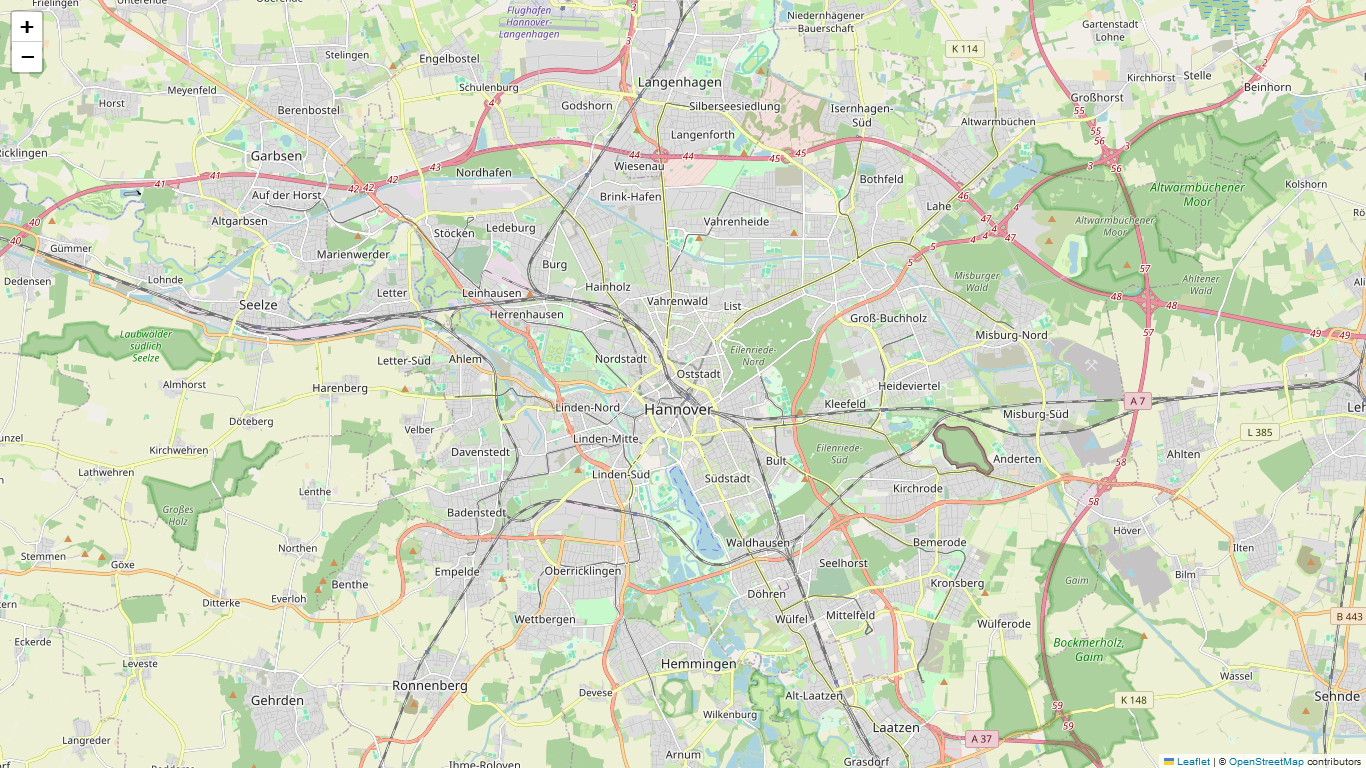
\includegraphics[keepaspectratio]{images/museumsmap_hannover.png}}

\part{Room}

\chapter{Bau-, Ausstattungs- und
Funktionsgeschichte}\label{bau--ausstattungs--und-funktionsgeschichte}

Die hervorragend erhaltene wandfeste Ausstattung des Großen Saals, der
1639 als „großer Saahl`` {[}1{]} geführt wurde und seinen heute
geläufigen Namen Rittersaal erst im Nachhinein erhielt, datiert aus den
Jahren 1601 bis 1605. Am Beginn stand den Quellen zufolge der
monumentale Saalkamin. Der Vertrag mit dem Bildhauer Michael Juncker aus
Miltenberg datiert vom 7. September 1601.{[}2{]} Im November 1601 wurden
mit Balthasar Katzenberger die Deckengemälde verdingt, der die Arbeiten
13 Monate später Anno 1602 abschloss.{[}3{]} 1603 signierte und datierte
der Kalkschneider Gerhard Schmidt das Portal an der inneren
Ostseite.{[}4{]} Die Jahreszahl 1605 zusammen mit den Initialen CL für
den Kalkschneider Christoph Limmerich über der Tür zum Altan markieren
den Abschluss der Arbeiten.{[}5{]}

Seit 1710/11 wurde der Saal unter Graf Carl Ludwig behutsam dem barocken
Zeitgeschmack angepasst und inhaltlich vom Jagd- zum gräflichen
Rittersaal umgedeutet. Christian Thalwitzer hatte Balthasar
Katzenbergers Deckengemälde „im großen Saal {[}zu{]} übermahlen, genau
durch{[}zu{]}gehen und wo es Schaden genommen, mit allem Fleyß``
auszubessern.{[}6{]} Bei dieser Gelegenheit versah er die Gemälderahmen
und die dazwischenliegenden Stuckrippen mit der bis heute gültigen roten
Marmorierung.{[}7{]} An den Wänden wurden die Roll- und
Beschlagwerkkartuschen der Schmuckzone ebenfalls rot marmoriert und an
Kamin und Innenportal die rot marmorierten Schattenrahmen hinzugefügt.

In einem zweiten Schritt wurde der Sockel ringsum mit rot marmorierten
Lambris versehen, die Christian Thalwitzer im Rechnungsjahr 1715/16 mit
51 Schloss- und Gartenveduten im Querformat{[}8{]} und 27 Orangenbäumen
und anderen exotischen Kübelpflanzen im Hochformat bemalte. Die 12
ganzfigurigen Porträts männlicher Vorfahren zum Teil in Ritterrüstung,
die dem Rittersaal seinen heutigen Namen gaben, schuf bereits 1710 Peter
Franz Tassaert aus Rothenburg.{[}9{]}

\section{\texorpdfstring{\textbf{Beschreibung des
Raumes}}{Beschreibung des Raumes}}\label{beschreibung-des-raumes}

Der 36,4 Meter lange, 11,7 Meter breite und 8,25 Meter hohe Saal{[}10{]}
wird durch hohe segmentbogenförmige Fensternischen gegliedert, deren
Achsen von großen Okuli weitergeführt werden. Im Gegenzug zu dieser
Vertikalen beschränkt sich der reiche Stuckdekor friesartig auf die
obere Wandzone, die oberhalb eines Gesimses auf der Höhe des oberen
Drittels der Fenster beginnt. Dadurch, dass sich die Stuckdekoration in
das obere Drittel der Fensterlaibungen hineinzieht, erwecken sie den
Eindruck hoheitsvoll gestelzter Bögen.{[}11{]}

An der Westwand, neben der im ersten Joch der Hofseite der Saal über die
Wendeltreppe betreten wird, erhebt sich ein monumentaler Kamin. Mit
Kaminöffnung, Attikafeld und rundbogigem Auszug umfasst er drei Zonen,
von denen Attika und Auszug in der Höhe der stuckierten Wandzone des
Saals entsprechen. An der Ostwand, wo man den Saal Richtung Tafelstube
verlässt, befindet sich ein prächtiges, 1603 datiertes stuckiertes
Innenportal des Kalkschneiders Gerhard Schmidt.{[}12{]} Darüber
verläuft, teilweise hinter dem Attikarelief, eine Empore beispielsweise
für Musiker.

Den Kamin flankieren stuckierte Darstellungen des Grafenpaars Wolfgang
II. von Hohenlohe und Magdalena, geborene Prinzessin von
Nassau-Katzenelnbogen mit ihrer jeweiligen Ahnenprobe.{[}13{]} Dem Graf
wurde die zeremoniell höherrangige Seite heraldisch rechts des Kamins,
der Gräfin die Seite heraldisch links des Kamins zugeteilt. Graf und
Gräfin liegen jeweils auf der Seite einander abgewandt und blicken mit
aufgestütztem Kopf in den Saal. Aus ihnen heraus wächst in der Art einer
Wurzel Jesse die über fünf Generationen geführte Ahnenprobe. Der Graf
trägt eine Rüstung mit Waffenrock und stützt seinen Ellenbogen auf einen
Helm. Die Gräfin hat zwei Kinder im Arm, von denen das vordere ein Junge
ist.

An den beiden Längsseiten nimmt die stuckierte Schmuckzone weit
vorkragende, gleichfalls stuckierte Wandskulpturen wilder Tiere auf. Sie
beziehen sich einerseits auf das Programm der Decke, das der höfischen
Jagd in all ihren Ausformungen gewidmet ist. Andererseits sind sie auf
die Kaminwand ausgerichtet, die mit ihren nachstehend zu erläuternden
Bildthemen als Stellvertreter des Grafen, seiner konfessionellen
Einstellung und seiner dynastischen Herkunft konzipiert ist. Zusammen
mit einer gemalten Darstellung des lyraspielenden Orpheus an der Decke
erlauben die Tiere in ihrer Ausrichtung auf den Kamin die Identifikation
des Grafen mit Orpheus als Sinnbild des guten Herrschers. Diese hier
erstmals entwickelte Deutung wird unten im Abschnitt „Programm und
Synthese der Saalausstattung der Renaissance`` vorgetagen.

\section{Kamin und Innenportal}\label{kamin-und-innenportal}

Der Kamin aus Andernacher Tuffstein von Michael Juncker und seinen
Söhnen Hans und Zacharias aus Miltenberg präsentiert im Hauptrelief als
zentrales Motiv die persönliche Devise des Grafen Wolfgang. Die
Entschlüsselung der im Vertrag vom September 1601 vereinbarten „ihrer
gnaden Diviso``{[}14{]} gelang erst vor wenigen Jahren Jürgen
Kniep.{[}15{]} Dargestellt ist ein antikisch gekleideter Krieger,
umgeben von den Symbolen der Kardinal- und theologischen Tugenden. Die
Devise „Gott gibt Glück`` lässt den reformatorischen Glauben des Grafen
Wolfgang ebenso erkennen wie die Betonung der Liebe (Herz in der linken
Hand des Kriegers) und des Buches, aus dem die Schlange ihre Weisheit
bezieht. Im Sinne der protestantischen Rechtfertigungslehre oblag es
nicht dem Klerus, sondern allein Gott, dem Menschen Gnade angedeihen zu
lassen.

Als räumliches Gegenstück zum skulptierten Kamin entstand 1603 in einem
Paragone der Techniken und Materialien das monumentale, aus Stuck
gefertigte Innenportal an der Ostseite. Sein Aufbau ist wie der Kamin
dreizonig mit rundbogiger Öffnung, Attikarelief und Auszug. Der
Kalkschneider Gerhard Schmidt, der das Portal selbstbewusst mit seinen
Initialen signiert hat, hat in der Türkenschlacht des Hauptreliefs mit
extrem hinterschnittenen Pferde- und Soldatenleibern den moderater
skulptierten Steinkamin an Kunstfertigkeit übertroffen. Einen Höhepunkt
der Stuckateurskunst der Zeit bildet der vollplastisch gearbeitete
heilige Georg auf seinem zum Sprung über den Drachen ansetzenden Pferd.

Das Portal ist inhaltlich auf den ältesten Sohn des Grafen Wolfgang,
Georg Friedrich, zu beziehen, der im Rang eines Obristen des Fränkischen
Reichskreises und auch der kaiserlichen Armee im Langen Türkenkrieg
(1593--1606) kämpfte.{[}16{]} Als einer seiner größten Erfolge gilt die
versuchte Einnahme der Festung Gran (Eszergom) im Jahr 1594, an der er
als kaiserlicher Obrist beteiligt war.{[}17{]} Die Festung, vor der sich
auf dem Relief das Schlachtengetümmel abspielt, stellt in der Tat
Eszergom da, was an der Höhenlage und der Zweiturmfassade der Kathedrale
zu erkennen ist.{[}18{]} Der das Portal bekrönende heilige Georg als
Drachentöter mit Lanze und zugleich Namenspatron des Erbprinzen sowie
Patron der Stadtkirche wäre im Sinne des Protestantismus als
tugendhafter Bezwinger des Bösen zu deuten.{[}19{]} Mit der Thematik des
Langen Türkenkriegs bereitete das Portal auf die dahinterliegende
Tafelstube vor, für deren Decke Balthasar Katzenberger 12 große
Belagerungsszenen auf Leinwand malte.

Das Portal von 1603 war aber nicht nur heroisch gestimmt. In den
Zwickeln lagern Putti, die als Mahnung an die Endlichkeit des Lebens dem
Betrachter ein Stundenglas, eine Sense und einen Schlüssel -- vielleicht
ins Himmelreich -- vor Augen halten.

\section{Das Mobiliar}\label{das-mobiliar}

Die renaissancezeitliche Ausstattung des Saals mit Mobilien geht aus
einem 1625--1627 aufgenommenen Inventar hervor.{[}20{]} Die als erstes
genannten „Ein und zwanzig Stuck goldt uf Leder tappezerey`` dürften als
goldgeprägte Ledertapeten die Trumeaus zwischen den Fenstern geziert
haben. Ledertapeten waren kostbar, was sich in ihrer erstplatzierten
Nennung niederschlug.{[}21{]} An Stellmöbeln beinhaltete der Saal „Zwo
lange Tafel`` und „Ein und dreissig von goldt uff Lederne Sessel``. Die
Wände schmückten zusätzlich zu den Ledertapeten „Sechzehn gemahlte
Tafeln``, also im Sujet nicht näher charakterisierte Gemälde. Die
Beleuchtung erfolgte über „Acht große hülzerne Lichter, gemahlt``.

Vier Gemälde wurden zusätzlich zu den sechzehn aufgeführt, da sie
vermutlich im Vorgängerinventar des Grafen Wolfgang, das dem Inventar
als Vorlage diente, noch nicht enthalten waren. Sie stellten „Kaiser
Matthie und der Kayserin / Item Meines Gnd. Herrn und gnl. Frawen
Abcontrafehung`` dar. Kaiser Matthias regierte in den Jahren 1612--1619,
seine Gemahlin Anna von Österreich-Tirol starb 1618. Die Gemälde
stammten demnach aus der Zeit des Grafen Georg Friedrich von
Hohenlohe-Weikersheim, der mit Eva von Waldstein verheiratet war.

{[}1{]} HZAN La 130 Bü 152, Schadensinventar von 1639. Die Kenntnis und
die Transkription dieser Archivalie verdankt die Autorin Frieder
Leipold.

{[}2{]} Der erhaltene Vertrag (HZAN We 50 D6) in Transkription bei
Freeden, Kamin, 1950, S. 144--145. Bezahlt wurde Juncker im Oktober
1602.

{[}3{]} Poser, Deckenbilder, 1980, S. 160--161.

{[}4{]} Merten, Weikersheim, o. J., S. 44. Drös, Inschriften
Mergentheim, 2002, S. 244. Zum Oeuvre und Lebensweg des Kalkschneiders
Gerhard Schmidt: Kreder, Hellenstein, 2005/2006; Rinn-Kupka, Stuck,
2018, S. 126--129; Lange, ‚welsche Kamin`, 2019.

{[}5{]} Merten, Weikersheim, o. J., S. 44. Drös, Inschriften
Mergentheim, 2002, S. 254.

{[}6{]} Fandrey, Weikersheim, 2010, S. 55.

{[}7{]} Dieser Befund kam bei der Restaurierung der Jahre 1995--1997
zutage. Für zahlreiche Informationen und die Übermittlung des
Abschlussberichts vom 05.03.1998 dankt die Autorin Herrn Dipl.-Ing. Erik
Reinhold, Staatliches Hochbauamt Heilbronn.

{[}8{]} Die Vedute des Carlsberg bei Weikersheim kam erst 1747 im
Zusammenhang mit der damals aufgestellten Kunstuhr hinzu, doch dürfte
sie eine ältere Vedute am Fensterpfeiler hinter der Uhr ersetzt haben.

{[}9{]} Valentin, Malerische Lebensläufe, 2019, Anm. 11. Zu Tassaert
liegt ein Lebenslauf mit Werkverzeichnis vor: Schnurrer, Tassaert, 2014.

{[}10{]} Die genauen Maße gibt Walther-Gerd Fleck (Weyer, Georg Stegle,
2017, S. 52).

{[}11{]} Vgl. dagegen Gebeßler, Saal Süddeutschland, 1957, S. 49, der
die Fensternischen aufgrund ihrer Dekoration als Anräume empfindet.

{[}12{]} Das Portal wird in der Literatur zu Unrecht als Eingangsportal
in den Saal beschrieben (Poser, Deckenbilder, 1980, S. 160; Kniep,
Glück, 2005, S. 52 und 59; Käpplinger, Jagd, 2011, S. 73). Es ist jedoch
nach innen gerichtet, führt also von innen nach außen. Außerdem folgt in
der Wegeführung eines Renaissanceschlosses die Tafelstube auf den
Rittersaal. Auch der Betrachterstandpunkt der Deckengemälde ist mit dem
Rücken zum Kamin so ausgerichtet, dass man die Bilder vom Kamin kommend,
Richtung Tafelstube gehend bewundert.

{[}13{]} Zu den Ahnenproben: Drös, Inschriften Mergentheim, 2002, S.
255--261. Außerdem Kniep, Glück, 2005, S. 48--52.

{[}14{]} Freeden, Kamin, 1950, S. 144.

{[}15{]} Kniep, Glück, 2005, S. 57--74. Weiterführende Gedanken und
Literatur zur Bildhauerfamilie Juncker liefert: Lange, ‚welsche Kamin`,
2019.

{[}16{]} Kniep, Glück, 2005, S. 52--57. Außerdem Findbuch HZAN La 130 Bü
102 (Bestallung zum Obristen des Fränkischen Reichskreises, 1598) und La
130 Bü 108 (Teilnahme als kaiserlicher Obrist am Feldzug gegen die
Türken 1603).

{[}17{]} Trentin-Meyer, Georg Friedrich von Hohenlohe, 2019, S. 90. Vgl.
Niederkorn, Langer Türkenkrieg, 1993, S. 11.

{[}18{]} Außerdem als Beleg die Darstellung in: Ortelius, Chronologia,
1602, Tf. „Wahre Contrafactur der Belagerung Gran, sampt der Schlacht so
dabei geschehen, den 3. Augusti. Anno 1595``. Ortelius wählte für seine
Illustration die erfolgreiche Belagerung und Schlacht von 1595. Die
Belagerung von 1594 war für die Kaiserlichen noch nicht erfolgreich.

{[}19{]} Kniep, Glück, 2005, S. 56.

{[}20{]} Auszüge des Inventars stellte freundlicherweise Dinah
Rottschäfer der Autorin zur Verfügung.

{[}21{]} Bei dem von Käpplinger, Auf's Schönste, 2019, S. 189 mit Anm. 3
genannten Inventar von 1634 handelt es sich um einen Schadensbericht, in
dem die Ledertapeten verkürzt als „tappezereien von gold`` bezeichnet
wurden, was Käpplinger in Unkenntnis des Vorgängerinventars als textile
Wandbespannungen deutete.

\chapter{Gallery Full Image}\label{gallery-full-image}

\phantomsection\label{infogrid}
\phantomsection\label{paintingName}

\phantomsection\label{paintingYear}

\phantomsection\label{paintingSize}{} {Wikidata}

\chapter{List of Items}\label{list-of-items}

\begin{itemize}
\tightlist
\item
  a
\item
  b
\item
  c
\item
  d
\item
  e
\end{itemize}

\chapter{Sources \& Data Models}\label{sources-data-models}

\begin{itemize}
\tightlist
\item
  f
\item
  g
\item
  h
\item
  i
\item
  j
\item
  k
\end{itemize}

\chapter{Data Visualisation}\label{data-visualisation}

text

text

text


\backmatter

\printindex

%  SOURCE: https://github.com/nmfs-opensci/quarto_titlepages_v1/tree/main

% This is a combination of Pandoc templating and LaTeX
% Pandoc templating https://pandoc.org/MANUAL.html#templates

\tcbset{ % parameters for text background 
    frame code={},
    left=0pt, % margins
    right=0pt,
    top=0pt,
    bottom=0pt,
    colback=gray!10!black, % box color
    width=\dimexpr\textwidth\relax, 
    boxsep=15pt, % spacing between boxes
    arc=0pt, % no rounded edges
    opacityback=0.35, % translucent-ish background
    fontupper=\color{white}, % fontcolor
    fontlower=\color{white}
    }



% background image
  \ThisLRCornerWallPaper{1.1}{images/fmd10024322a.jpg}  

\bigbreak




%use \vfill instead to get the space to fill flexibly	
%\vspace{0.25\textheight} % Whitespace between the title block and the publisher

\vfill

% Whitespace between the title block and the tagline
\vspace{1\baselineskip} 

\begin{tcolorbox}
\centering

%%%%%% Tagline at bottom
{
  TIB\\
  Open Science Lab
}
\end{tcolorbox}


\end{document}
